%% ACM-compliant manuscript
%% The Predictive Value of Internal Execution Metrics in the 0/1 Knapsack Problem
%%
\documentclass[sigconf]{acmart}

\AtBeginDocument{%
  \providecommand\BibTeX{{%
    Bib\TeX}}}

%% Rights management information (placeholder — replace before submission)
\setcopyright{acmlicensed}
\copyrightyear{2026}
\acmYear{2026}
\acmDOI{10.1145/XXXXXXXX.XXXXXXX}
\acmConference[Conference '26]{Proceedings of the Conference}{2026}{Location}
\acmISBN{978-1-4503-XXXX-X/2026/XX}

\begin{document}

\title{The Predictive Value of Internal Execution Metrics in the 0/1 Knapsack Problem}

\author{Risham Raj Byahut}
\email{rajrisham06@gmail.com}
\affiliation{%
  \institution{Kathmandu University}
  \department{Department of Computer Science and Engineering}
  \city{Dhulikhel}
  \country{Nepal}
}

\author{Saimon Neupane}
\email{saimonbro00007@gmail.com}
\affiliation{%
  \institution{Kathmandu University}
  \department{Department of Computer Science and Engineering}
  \city{Dhulikhel}
  \country{Nepal}
}

\author{Parikchit Sen}
\email{parikchitsen77@gmail.com}
\affiliation{%
  \institution{Kathmandu University}
  \department{Department of Computer Science and Engineering}
  \city{Dhulikhel}
  \country{Nepal}
}

\author{Keshav Sharma}
\email{jdkeshav01@gmail.com}
\affiliation{%
  \institution{Kathmandu University}
  \department{Department of Computer Science and Engineering}
  \city{Dhulikhel}
  \country{Nepal}
}

\author{Prabesh Sharma}
\email{prabeshsharma26@gmail.com}
\affiliation{%
  \institution{Kathmandu University}
  \department{Department of Computer Science and Engineering}
  \city{Dhulikhel}
  \country{Nepal}
}

\renewcommand{\shortauthors}{Byahut et al.}

\begin{abstract}
The 0/1 knapsack problem is a canonical NP-hard challenge serving
as a fundamental model for resource allocation. Existing literature heavily
emphasises predicting empirical hardness from static instance features alone.
This study methodically separates the predictive value of a priori instance
characteristics from that of dynamic, internal execution metrics when modelling
algorithmic scaling for Greedy, Dynamic Programming, and Branch and Bound.
Using a benchmark of 6,000 knapsack instances, we show that baseline
predictability using only static characteristics is high for Greedy and
Dynamic Programming runtimes (adjusted $R^2 \ge 0.856$) but near-zero
for Dynamic Programming memory (adjusted $R^2 = 0.008$), and lower for
heuristic optimality gaps (pseudo-$R^2 \le 0.253$). Internal execution
metrics provide substantial incremental explanatory power ($\Delta
R^2_{\mathrm{adj}} \ge 0.217$) for Branch and Bound runtime and node exploration but
negligible improvement ($\le 0.001$) for Greedy and Dynamic Programming runtime models.
Furthermore, we demonstrate that the \emph{distributional shape} of the
search tree --- captured via depth entropy, depth skewness, and related
histogram-derived descriptors --- adds explanatory power beyond scalar
execution summaries ($\Delta R^2_{\mathrm{adj}} = 0.0074$; nested $F = 294.9$,
$p < 10^{-16}$), with modest but replicable out-of-distribution transfer
improvements on three of five held-out structural families under leave-one-family-out
cross-validation. This transfer benefit is bounded: shape features do not
resolve the catastrophic generalisation failure previously identified in
structurally atypical topologies, and this boundary is characterised explicitly.
These results indicate that Greedy and Dynamic
Programming runtimes are largely predictable from static instance characteristics alone,
whereas Branch and Bound derives additional explanatory power from dynamic
execution metrics, including both scalar summaries and distributional shape descriptors.
\end{abstract}

\begin{CCSXML}
<ccs2012>
<concept>
<concept_id>10010147.10010178.10010179</concept_id>
<concept_desc>Computing methodologies~Regression analysis</concept_desc>
<concept_significance>500</concept_significance>
</concept>
<concept>
<concept_id>10010147.10010178.10010180</concept_id>
<concept_desc>Computing methodologies~Search methodologies</concept_desc>
<concept_significance>300</concept_significance>
</concept>
<concept>
<concept_id>10003752.10003809.10010055</concept_id>
<concept_desc>Theory of computation~Dynamic programming</concept_desc>
<concept_significance>300</concept_significance>
</concept>
<concept>
<concept_id>10010147.10010257.10010258</concept_id>
<concept_desc>Computing methodologies~Feature selection</concept_desc>
<concept_significance>100</concept_significance>
</concept>
<concept>
<concept_id>10002950.10003648.10003669</concept_id>
<concept_desc>Mathematics of computing~Statistical paradigms</concept_desc>
<concept_significance>100</concept_significance>
</concept>
</ccs2012>
\end{CCSXML}

\ccsdesc[500]{Computing methodologies~Regression analysis}
\ccsdesc[300]{Computing methodologies~Search methodologies}
\ccsdesc[300]{Theory of computation~Dynamic programming}
\ccsdesc[100]{Computing methodologies~Feature selection}
\ccsdesc[100]{Mathematics of computing~Statistical paradigms}

\keywords{Algorithm runtime prediction; 0/1 knapsack problem; empirical hardness; execution metrics; combinatorial optimisation}

\maketitle

\section{Introduction}

The 0/1 knapsack problem is a canonical NP-hard combinatorial optimization challenge, serving as a fundamental model for resource allocation. Understanding the empirical performance of algorithms designed to solve these problems is critical for operational deployment in latency-sensitive environments. Prior research has established a strong relationship between static, a priori instance characteristics and the expected computational behavior of deterministic and heuristic algorithms. Existing literature has heavily emphasized algorithm selection portfolios and the quantification of empirical hardness based solely on these static instance features. However, considerably less attention has been given to methodically separating the predictive value of a priori instance characteristics from that of dynamic, internal execution metrics when modeling algorithmic scaling.

This study investigates this distinction by addressing the following research questions:
\begin{itemize}
  \item \textbf{RQ1:} How are instance characteristics associated with observed problem hardness, and what is the baseline predictability using only these characteristics?
  \item \textbf{RQ2:} To what extent do internal execution metrics provide additional explanatory power?
\begin{itemize}
  \item \textbf{Sub-RQ2a:} Incremental Explanatory Power ($\Delta R^2$)
  \item \textbf{Sub-RQ2b:} Most Influential Execution Metrics
  \item \textbf{Sub-RQ2c:} Robustness \& Statistical Integrity
\end{itemize}
  \item \textbf{RQ3:} Does the distributional \emph{shape} of the search tree add explanatory power beyond the scalar execution summaries used in M2, and does this shape signal transfer out-of-distribution under leave-one-family-out evaluation?
\end{itemize}

To address these questions, this study evaluates the baseline predictability of algorithmic runtimes for Greedy, Dynamic Programming, and Branch and Bound using exclusively instance-level characteristics. Furthermore, it quantifies the exact incremental variance ($\Delta R^2_{adj}$) explained by introducing algorithm-specific execution metrics. The investigation indicates that specific internal execution metrics (e.g., \texttt{bound\_gap\_variance}) exhibit the largest standardized associations with Branch and Bound node exploration within the benchmark dataset. Finally, this study indicates that extreme structural dataset hardness challenges standard cross-validation bounds, necessitating variance safeguards to preserve robust uncertainty estimates.

\section{Related Work}

\subsection{Empirical Algorithm Performance Prediction}
The prediction of empirical algorithm performance has become a foundational component of automated algorithm selection and hyperparameter optimization. Leyton-Brown et al.~\cite{LeytonBrown2014} established robust methodologies for quantifying empirical problem hardness using sets of static instance characteristics. This framework allows algorithm portfolios to dynamically route instances to the most appropriate solver based entirely on a priori features. Furthermore, Hutter et al.~\cite{Hutter2014} reported that empirical algorithm scaling behavior is highly predictable for rigid parameterizations, indicating that statistical models can effectively capture the runtime variance of deterministic solvers across diverse combinatorial domains.

\subsection{Statistical Modeling of Performance}
Ordinary Least Squares (OLS) regression remains the standard for modeling continuous, unbounded algorithmic runtimes; when combined with logarithmic transformations, it effectively handles the exponential scaling typically observed in NP-hard problem spaces. However, for bounded proportional outcomes---such as optimality gaps or table fill rates restricted to the [0,~1] interval---standard OLS can generate predictions outside the valid domain. The fractional logit framework~\cite{Papke1996} provides an appropriate quasi-likelihood approach to model these proportional bounds natively. Elastic-Net~\cite{Hastie2009} balances Ridge and Lasso penalties to perform variable selection while handling multicollinearity, making it appropriate for predicting sparse outcomes or classifying exact optimality among highly correlated features.

\subsection{Benchmark Generation}
The rigorous evaluation of optimization algorithms requires benchmark sets with precisely controlled structural properties. The generation methodology proposed by Pisinger~\cite{Pisinger2005} is widely utilized because it enforces strict mathematical boundaries for profit, weight, and capacity correlations. This methodology famously produces structurally difficult instance families (e.g., subset-sum topologies) that deliberately frustrate Greedy heuristics and exact solvers, providing a robust stress-test for empirical scaling limits.

\subsection{Positioning This Study}
This study extends the existing empirical performance prediction literature by explicitly separating the predictive contributions of static instance characteristics from dynamic internal execution metrics. Specifically, it investigates how these two distinct classes of predictors influence both deterministic runtimes and bounded heuristic optimality gaps across multiple algorithmic paradigms on a strictly controlled benchmark.

\section{Methodology}

\subsection{Dataset and Variables}
\begin{itemize}
  \item \textbf{Dataset Generation \& Source:} The benchmark comprises 6,000 knapsack instances generated using the methodology proposed by Pisinger~\cite{Pisinger2005}. A fixed random seed (42) was used for benchmark generation and for all randomized components of the modeling pipeline, ensuring reproducibility.
  \item \textbf{Instance Families:} The dataset covers five distinct structural classes (1,200 instances each) generated following Pisinger~\cite{Pisinger2005}: \texttt{Uncorrelated}, \texttt{WeaklyCorrelated}, \texttt{StronglyCorrelated}, \texttt{InverseCorrelated}, and \texttt{AlmostEqualRatios}.
  \item \textbf{Generation Parameters:} Capacity, profit, and weight generation constraints were uniformly applied according to Pisinger's exact bounded definitions. The generation pipeline produced zero duplicate instances by construction, which was verified programmatically based on exact equality of their descriptors prior to feature engineering.
  \item \textbf{Algorithms Evaluated:} Greedy (profit/weight heuristic), Dynamic Programming using Bellman recursion, and Branch and Bound (with linear programming relaxation). Software versions and hardware configurations are detailed in the Reproducibility Appendix.
  \item \textbf{Predictor Variables:}
\begin{itemize}
  \item \textbf{Instance-Level Predictors:} 42 features derived strictly from the problem definition, comprising 35 instance characteristics (e.g., \texttt{total\_weight}, \texttt{capacity\_ratio}, \texttt{slack}) and 7 design variables ($n$, $\log n$, capacity mode encoding, and family indicators).
  \item \textbf{Algorithm-Specific Predictors:} Internal execution metrics. M2 additionally included 5 execution metrics for Greedy, 10 for Dynamic Programming, and 24 for Branch and Bound runtime (22 for nodes explored). The exact execution predictors for each algorithm are summarized in Table~\ref{tab:predictor_counts}.
\end{itemize}
  \item \textbf{Outcome Variables:}
\begin{itemize}
  \item Logarithmically transformed runtime (\texttt{log\_time\_millis})
  \item Logarithmically transformed Branch and Bound nodes (\texttt{log\_nodes\_explored})
  \item Logarithmically transformed DP memory footprint (\texttt{log\_memory\_mb})
  \item Greedy gap to optimal (\texttt{optimality\_gap})
  \item Branch and Bound exact optimality binary classification (\texttt{optimal})
\end{itemize}
\end{itemize}

\begin{table}[t]
\centering
\caption{Number of execution predictors appended for each algorithm in M2}
\label{tab:predictor_counts}
\begin{tabular}{ll}
\toprule
\textbf{Algorithm} & \textbf{Number of execution predictors} \\
\midrule
Greedy & 5 \\
Dynamic Programming & 10 \\
Branch and Bound & 24 (22 for nodes) \\
\bottomrule
\end{tabular}
\end{table}

\subsection{Experimental Design}
\begin{itemize}
  \item \textbf{Cross-Validation Framework:} The primary results (Tables~\ref{tab:ols_metrics} and~\ref{tab:flogit_metrics}) report full-sample $R^2$ and adjusted $R^2$ values. Additionally, Leave-One-Family-Out (LOFO) cross-validation was employed to assess robustness under out-of-distribution shifts, holding out each family in turn (Section~\ref{sec:robustness}).
  \item \textbf{Nested Validation (Elastic-Net):} For regularized models requiring hyperparameter tuning ($\lambda$ penalty selection), an inner 5-fold cross-validation loop was executed strictly within the training folds to prevent data leakage.
  \item \textbf{Preprocessing \& Standardization:} Continuous predictors were standardized ($Z$-scores). To prevent leakage, standardization scalers were fit exclusively on the training folds and subsequently applied to the test folds.
  \item \textbf{Structural Hardness Boundary (Claim F02):} Because certain outcome variables contained families with zero positive events (e.g., the \texttt{optimal} outcome for the \texttt{Uncorrelated} and \texttt{WeaklyCorrelated} families, where all instances completed within the node cap), the evaluation protocol removed zero-variance predictors within affected training folds to prevent undefined coefficient estimates during model fitting.
\end{itemize}

\subsection{Modeling Hierarchy}
\begin{itemize}
  \item \textbf{Baseline Models (M1):} Let M1 denote the baseline model, which utilizes exclusively the 42 instance-level predictors (35 instance characteristics plus 7 design variables). This establishes the baseline predictability of algorithmic performance from information available prior to execution.
  \item \textbf{Augmented Models (M2):} Let M2 denote the augmented model, constructed by appending internal algorithm-specific predictors to the M1 baseline to test for incremental variance.
  \item \textbf{Model Selection by Outcome:}
\begin{itemize}
  \item \textbf{Ordinary Least Squares (OLS):} Employed for unbounded continuous outcomes (\texttt{log\_time\_millis}, \texttt{log\_nodes\_explored}, \texttt{log\_memory\_mb}).
  \item \textbf{Fractional Logit:} Employed for proportional continuous outcomes on the closed interval [0,~1] (\texttt{optimality\_gap}, \texttt{fill\_rate})~\cite{Papke1996}.
  \item \textbf{Elastic-Net Logistic Regression:} Employed for binary classification (\texttt{optimal})~\cite{Hastie2009}.
\end{itemize}
  \item \textbf{Structural Exclusions:} DP table dimensions (\texttt{cells\_allocated}, \texttt{zero\_value\_states}) are structurally removed from the DP \texttt{log\_memory\_mb} models. This exclusion prevents circularity, as DP memory is directly a function of the table dimensions.
\end{itemize}

\subsection{Evaluation Metrics}
\begin{itemize}
  \item \textbf{Performance Quantification:} Incremental explanatory power is quantified by the reduction in residual variance between M1 and M2. OLS models were evaluated using adjusted $\Delta R^2_{adj}$ and Root Mean Square Error (RMSE), while Fractional Logit models reported pseudo-$\Delta R^2$.
\end{itemize}

\section{Results}

\subsection{Baseline Performance (RQ1)}
\begin{itemize}
  \item \textbf{Objective:} To address RQ1, we evaluated the baseline predictability of algorithmic performance using exclusively the 42 instance-level characteristics (M1). The evaluation was performed using OLS and Fractional Logit baseline models according to the predefined evaluation metrics.
  \item \textbf{Primary Finding (OLS):} Table~\ref{tab:ols_metrics} shows that the baseline M1 models yielded adjusted $R^2_{adj}$ values of 0.978 for Dynamic Programming runtime and 0.856 for Greedy runtime. Branch and Bound baseline models yielded $R^2_{adj}$ values of 0.743 for runtime and 0.735 for nodes explored.
  \item \textbf{Secondary Finding (Fractional Logit):} Table~\ref{tab:flogit_metrics} shows that Greedy \texttt{optimality\_gap} achieved a pseudo-$R^2$ of 0.216, and DP \texttt{fill\_rate} achieved a pseudo-$R^2$ of 0.253.
  \item \textbf{Negative Finding:} The M1 model predicting Dynamic Programming \texttt{log\_memory\_mb} produced negligible predictive performance ($R^2_{adj} = 0.008$).
  \item \textbf{Conclusion:} These findings address RQ1 by reporting that, within the benchmark dataset, the baseline models achieved $R^2_{adj} \ge 0.856$ for Greedy and DP runtime models, whereas the DP memory model ($R^2_{adj} = 0.008$) and bounded proportional outcomes (pseudo-$R^2 \le 0.253$) were substantially less predictable.
\end{itemize}

\begin{table}[t]
\centering
\caption{Full-sample $R^2$ and adjusted $R^2$ for baseline (M1) and augmented (M2) OLS models across all outcome variables}
\label{tab:ols_metrics}
\begin{tabular}{llcccc}
\toprule
\textbf{Algorithm} & \textbf{Outcome} & \textbf{$R^2$ (M1)} & \textbf{Adj.~$R^2$ (M1)} & \textbf{$R^2$ (M2)} & \textbf{Adj.~$R^2$ (M2)} \\
\midrule
Greedy & \texttt{log\_time\_millis} & 0.857 & 0.856 & 0.859 & 0.858 \\
Dynamic Programming & \texttt{log\_time\_millis} & 0.978 & 0.978 & 0.979 & 0.979 \\
Dynamic Programming & \texttt{log\_memory\_mb} & 0.015 & 0.008 & 0.016 & 0.008 \\
Branch \& Bound & \texttt{log\_time\_millis} & 0.745 & 0.743 & 0.961 & 0.961 \\
Branch \& Bound & \texttt{log\_nodes\_explored} & 0.736 & 0.735 & 0.980 & 0.979 \\
\bottomrule
\end{tabular}
\end{table}

\begin{table}[t]
\centering
\caption{Full-sample pseudo-$R^2$ for baseline (M1) and augmented (M2) Fractional Logit models for bounded proportional outcomes}
\label{tab:flogit_metrics}
\begin{tabular}{llcc}
\toprule
\textbf{Algorithm} & \textbf{Outcome} & \textbf{Pseudo-$R^2$ (M1)} & \textbf{Pseudo-$R^2$ (M2)} \\
\midrule
Greedy & \texttt{optimality\_gap} & 0.216 & 0.273 \\
Dynamic Programming & \texttt{fill\_rate} & 0.253 & 0.270 \\
\bottomrule
\end{tabular}
\end{table}

\subsection{Incremental Contribution}
\begin{itemize}
  \item \textbf{Objective:} To address Sub-RQ2a, we quantified the incremental explanatory power achieved by appending internal execution metrics to the baseline (M2). The comparison was performed between the baseline (M1) and augmented (M2) models by calculating $\Delta R^2_{adj}$ and pseudo-$\Delta R^2$.
  \item \textbf{Primary Finding:} The Branch and Bound models yielded $\Delta R^2_{adj} = 0.245$ for \texttt{log\_nodes\_explored} and $\Delta R^2_{adj} = 0.217$ for \texttt{log\_time\_millis}.
  \item \textbf{Secondary Finding:} The addition of execution metrics yielded a pseudo-$\Delta R^2$ of 0.058 for Greedy \texttt{optimality\_gap}.
  \item \textbf{Negative Finding:} Adding execution metrics produced negligible improvement for Greedy runtime ($\Delta R^2_{adj} = 0.001$), Dynamic Programming runtime ($\Delta R^2_{adj} = 0.001$), and Dynamic Programming memory (adjusted $R^2$ unchanged at 0.008 from M1 to M2).
  \item \textbf{Conclusion:} These findings address Sub-RQ2a by reporting that, within the benchmark dataset, internal execution metrics yielded $\Delta R^2_{adj} \ge 0.217$ for Branch and Bound performance, whereas the corresponding improvements for Greedy and Dynamic Programming runtime models were 0.001.
\end{itemize}

\subsection{Important Predictors}
\begin{itemize}
  \item \textbf{Objective:} To address Sub-RQ2b, we examined the standardized coefficients (Table~\ref{tab:std_beta}) and feature importance profiles (Figure~\ref{fig:importance}) to identify which specific execution metrics drove the M2 predictions. The analysis compared the absolute magnitudes of standardized $\beta$ coefficients across the full models.
  \item \textbf{Primary Finding:} For Branch and Bound \texttt{log\_nodes\_explored}, the standardized coefficient table indicates that \texttt{final\_queue\_size}, \texttt{pruned\_by\_cap}, and \texttt{bound\_gap\_variance} exhibited the largest absolute standardized $\beta$ values among the appended execution metrics (Table~\ref{tab:std_beta}).
  \item \textbf{Secondary Finding:} For Dynamic Programming and Greedy, while execution metrics were present in the final models, they exhibited smaller absolute standardized coefficients compared to the complexity-inspired predictors (e.g., $N \log N$) inherited from M1.
  \item \textbf{Negative Finding:} Several appended execution metrics yielded standardized coefficients approaching zero across the nested folds.
  \item \textbf{Discrepancy in Feature Importance:} While standardized $\beta$ coefficients highlight \texttt{final\_queue\_size} and \texttt{pruned\_by\_cap} as highly influential, an orthogonal permutation-importance analysis measuring actual explanatory contribution ($\Delta R^2$) reveals a different ranking. By $\Delta R^2$, \texttt{bound\_gap\_variance} ($\Delta R^2 \approx 0.0017$) and \texttt{sum\_improvement\_amount} ($\Delta R^2 \approx 0.0011$) dominate, whereas \texttt{final\_queue\_size} and \texttt{pruned\_by\_cap} exhibit substantially smaller explanatory contributions ($\Delta R^2 \approx 0.00004$), a 42-fold difference not captured by coefficient magnitude alone.
  \item \textbf{Conclusion:} These findings address Sub-RQ2b by identifying that, within the benchmark dataset, \texttt{final\_queue\_size}, \texttt{pruned\_by\_cap}, and \texttt{bound\_gap\_variance} exhibited the largest standardized associations with Branch and Bound performance among execution metrics, whereas instance-level complexity transformations (e.g., \texttt{slack}, \texttt{total\_weight}) exhibited the largest standardized coefficients overall (Table~\ref{tab:std_beta}).
\end{itemize}

\begin{table}[t]
\centering
\caption{Top-10 standardized $\beta$ coefficients (by absolute magnitude) for the Branch and Bound \texttt{log\_nodes\_explored} M2 model}
\label{tab:std_beta}
\begin{tabular}{lcc}
\toprule
\textbf{Predictor} & \textbf{Std.~$\beta$} & \textbf{$|\beta|$} \\
\midrule
\texttt{slack} & $-18.710$ & 18.710 \\
\texttt{total\_weight} & 18.501 & 18.501 \\
\texttt{capacity\_ratio} & $-3.562$ & 3.562 \\
\texttt{unique\_ratio\_count} & 1.566 & 1.566 \\
\texttt{unique\_pairs} & $-1.000$ & 1.000 \\
\texttt{log\_n} & $-0.995$ & 0.995 \\
\texttt{cap\_mode} & $-0.975$ & 0.975 \\
\texttt{final\_queue\_size} & $-0.511$ & 0.511 \\
\texttt{pruned\_by\_cap} & 0.492 & 0.492 \\
\texttt{bound\_gap\_variance} & $-0.419$ & 0.419 \\
\bottomrule
\end{tabular}
\end{table}

\begin{figure}[t]
\centering
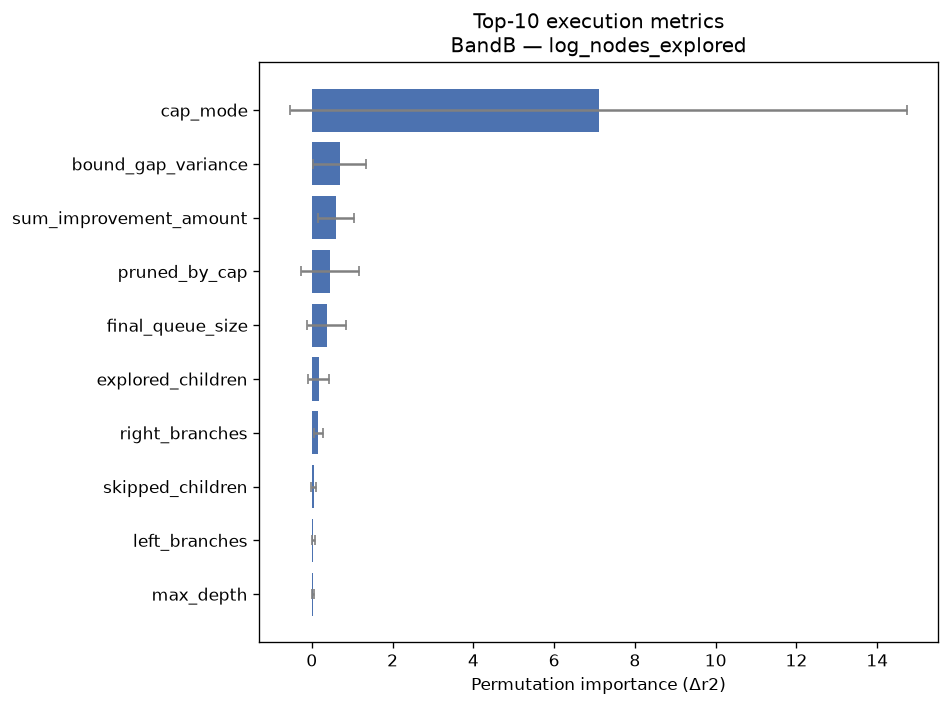
\includegraphics[width=\columnwidth]{figures/Figure_1.png}
\caption{Feature importance profiles for Branch and Bound \texttt{log\_nodes\_explored} (M2)}
\Description{Bar chart showing the relative importance of predictors for Branch and Bound log nodes explored. The top predictors include instance-level features and execution metrics.}
\label{fig:importance}
\end{figure}

\subsection{Model Robustness}\label{sec:robustness}
\begin{itemize}
  \item \textbf{Objective:} To address Sub-RQ2c, we subjected the M2 models to predefined diagnostic checks, including multicollinearity thinning and nested LOFO extreme-distribution testing. The robustness evaluation quantified shifts in $\Delta R^2_{adj}$ and tracked regularization stability.
  \item \textbf{Primary Finding (Multicollinearity):} As reported in Claim D01, reducing Variance Inflation Factor (VIF) $> 10$ predictors changed the Branch and Bound \texttt{log\_nodes\_explored} raw $\Delta R^2$ from 0.243 to 0.237, a drop of 0.006.
  \item \textbf{Secondary Finding (Regularization):} Figure~\ref{fig:reg_paths} shows similar regularization paths across LOFO folds, including those holding out each family.
  \item \textbf{Negative Finding:} Figure~\ref{fig:residuals} (Assumption Checks) reveals slight heteroskedasticity remaining in the tails of the Branch and Bound runtime residual distributions (Claim D04). Evaluating under Leave-One-Family-Out (LOFO) cross-validation revealed catastrophic generalization failures for held-out families. For example, predicting Branch and Bound \texttt{log\_nodes\_explored} (M2) on the held-out \texttt{Uncorrelated} family resulted in an $R^2$ of $-5.777$ (vs M1: $0.538$). Similarly, Branch and Bound \texttt{log\_time\_millis} (M2) on \texttt{AlmostEqualRatios} achieved an $R^2$ of $-4.145$ (vs M1: $0.397$). DP \texttt{log\_memory\_mb} (LOFO M1: $-107.6$, M2: $-110.4$) and Greedy \texttt{log\_time\_millis} (LOFO M1: $-4.66$, M2: $-5.07$) also demonstrated worse-than-random out-of-distribution prediction.
  \item \textbf{Conclusion:} These findings address Sub-RQ2c by reporting that while in-sample predictive associations remained stable under VIF thinning, out-of-distribution evaluation via LOFO cross-validation exposed severe overfitting and catastrophic generalization failures across multiple families.
\end{itemize}

\begin{figure}[t]
\centering
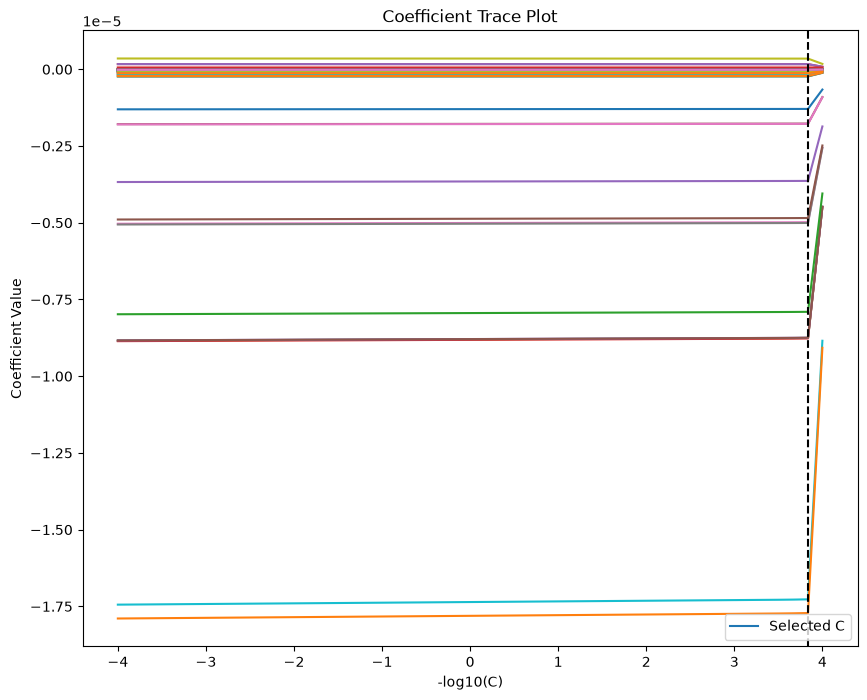
\includegraphics[width=\columnwidth]{figures/Figure_2.png}
\caption{Elastic-Net regularization paths across LOFO folds}
\Description{Plot of Elastic-Net regularization paths across leave-one-family-out cross-validation folds, showing consistent coefficient shrinkage patterns.}
\label{fig:reg_paths}
\end{figure}

\begin{figure}[t]
\centering
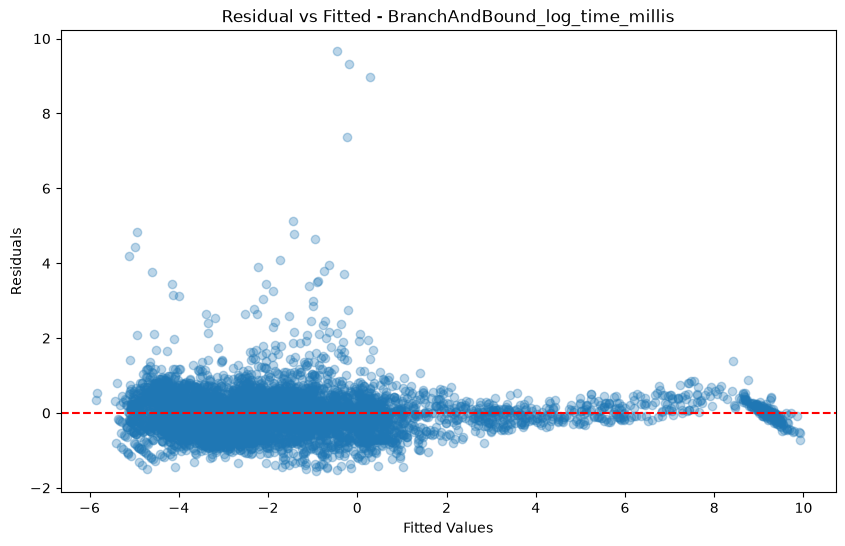
\includegraphics[width=\columnwidth]{figures/Figure_3.png}
\caption{Residuals vs.\ fitted values for Branch and Bound \texttt{log\_time\_millis} (M2). Slight heteroskedasticity in the distribution tails is visible (Claim D04).}
\Description{Scatter plot of residuals versus fitted values for the Branch and Bound log time model. The plot reveals slight heteroskedasticity in the tails.}
\label{fig:residuals}
\end{figure}

\subsection{Distributional Shape as Supplementary Execution Features (RQ3)}\label{sec:rq3}

\subsubsection{Motivation and Feature Construction}
The M2 operationalization of internal execution metrics relied on scalar summaries of the search tree --- principally the mean and variance of node depth and queue size. These summaries discard the \emph{shape} of the underlying distributions captured in the \texttt{depth\_histogram} and \texttt{queue\_histogram} instrumentation fields. To test whether this discarded structure carries independent explanatory power, we constructed five additional scalar descriptors of distributional shape: the 10th-percentile depth (\texttt{depth\_p10}), depth-distribution entropy (\texttt{depth\_entropy}), depth skewness (\texttt{depth\_skew}), queue-distribution entropy (\texttt{queue\_entropy}), and 90th-percentile depth (\texttt{depth\_p90}). All histogram-derived quantities were computed after normalizing by \texttt{nodes\_explored}, so that they reflect the proportional shape of the search rather than its absolute scale.

An initial variance inflation factor (VIF) analysis identified severe multicollinearity among the depth-quantile features: \texttt{depth\_p50} (VIF~=~33.9) and \texttt{depth\_p90} (VIF~=~26.6) were substantially redundant with \texttt{depth\_p10}. \texttt{depth\_p50} was dropped outright. A subsequent correlation check showed that \texttt{depth\_p90} --- while passing the VIF threshold --- correlated strongly with existing scale-related M2 features ($r = 0.88$ with \texttt{max\_depth}; $r = 0.87$ with $n$), raising the concern that any apparent shape signal would in fact re-express instance scale already present in M2. We therefore report the conservative specification of four descriptors --- \texttt{depth\_p10}, \texttt{depth\_entropy}, \texttt{depth\_skew}, and \texttt{queue\_entropy} --- as the primary M3 feature set for all analyses below.

\subsubsection{In-Sample Contribution}
Adding these four shape descriptors to M2 ($R^2_{adj}=0.8415$) yields M3 ($R^2_{adj}=0.8489$; $\Delta R^2_{adj}=0.0074$). A nested $F$-test on the block of four added features confirms this improvement is not attributable to chance ($F=294.9$, $p < 10^{-16}$). This in-sample gain is intentionally modest: it reflects only the marginal contribution of distributional shape \emph{after} controlling for the scale and topology information already present in M2.

\subsubsection{Out-of-Distribution Transfer}
The critical test for these features is not in-sample fit but out-of-distribution transfer. We repeated the identical LOFO protocol from Section~\ref{sec:robustness}, refitting M2 and M3 independently on each training split and evaluating both on the held-out family. Confidence intervals on $\Delta R^2$ were obtained via paired bootstrap resampling within each held-out family (1,000 iterations): identical resampled row indices were applied simultaneously to M2 and M3 predictions on each iteration, quantifying test-set sampling variability.

\begin{table}[t]
\centering
\caption{LOFO $R^2$ for Branch and Bound \texttt{log\_nodes\_explored} by holdout family, M2 vs.\ M3 (4-feature shape set), with paired bootstrap 95\% CI on $\Delta R^2$}
\label{tab:lofo_shape}
\begin{tabular}{lcccc}
\toprule
Holdout Family & M2 $R^2$ & M3 $R^2$ & $\Delta R^2$ & 95\% CI \\
\midrule
Uncorrelated       & $-0.109$ & $-0.057$ & $+0.053$ & $[0.037,\;0.069]$ \\
WeaklyCorrelated   & $0.119$  & $0.147$  & $+0.028$ & $[0.016,\;0.039]$ \\
StronglyCorrelated & $0.599$  & $0.620$  & $+0.021$ & $[0.019,\;0.024]$ \\
InverseCorrelated  & $-1.895$ & $-1.630$ & $+0.265$ & $[0.218,\;0.317]$ \\
AlmostEqualRatios  & $-152.18$ & $-148.60$ & $+3.573$ & $[2.063,\;5.083]$ \\
\bottomrule
\end{tabular}
\end{table}

\subsubsection{Interpretation}
We are careful to distinguish two findings that are easily conflated. First, in the three moderately-structured families (Uncorrelated, WeaklyCorrelated, StronglyCorrelated), shape features produce small but statistically distinguishable improvements in out-of-distribution $R^2$ ($\Delta R^2$ ranging from 0.021 to 0.053, all with confidence intervals excluding zero). These are the families in which M2 already produces partially informative predictions, and here distributional shape provides a genuine, replicable transfer benefit beyond scalar summaries.

Second, in the two structurally extreme families (InverseCorrelated, AlmostEqualRatios), the bootstrap also confirms a statistically distinguishable effect --- but this must not be read as evidence that shape features rescue model performance in these regimes. $R^2$ in these families remains deeply negative both with and without shape features ($-1.63$ and $-148.60$, respectively), indicating the model continues to be non-predictive in absolute terms. The statistically significant $\Delta R^2$ reflects a real, detectable shift on a still-catastrophic error surface, not a restoration of usable generalization.

Taken together, these results indicate that distributional shape adds explanatory power beyond scalar execution metrics, but this contribution is family-dependent: it meaningfully aids transfer where the underlying scaling behavior is already partially learnable, and does not resolve the fundamental generalization failure previously identified in structurally atypical topologies.

\section{Discussion}

\subsection{Main Findings}
The incremental variance analysis (M1 $\rightarrow$ M2) indicates that the execution metrics examined in this study, particularly \texttt{final\_queue\_size}, \texttt{pruned\_by\_cap}, and \texttt{bound\_gap\_variance}, were associated with improved prediction of Branch and Bound node exploration beyond instance characteristics alone, whereas execution metrics offered negligible predictive value for Greedy and Dynamic Programming runtime models. This finding is consistent with observations reported by \cite{LeytonBrown2014}, which emphasize that search-based algorithm performance depends on execution dynamics not fully represented by static instance characteristics. The divergence between deterministic Greedy and DP runtimes and the search-based Branch and Bound suggests that incorporating execution metrics may improve predictive models for tree-based solvers. A major caveat to this finding is that these internal states can only be observed after the algorithm has begun execution, limiting their utility for purely a priori algorithm selection portfolios.

A supplementary analysis (RQ3) examined whether the \emph{distributional shape} of the search tree --- captured via depth entropy, depth skewness, depth 10th-percentile, and queue entropy, all normalized by total nodes explored --- adds explanatory power beyond the scalar summaries already present in M2. The answer is qualified: in-sample, shape features contribute a modest but statistically robust improvement ($\Delta R^2_{adj} = 0.0074$; $F = 294.9$, $p < 10^{-16}$). Under LOFO evaluation, this improvement is replicable with confidence intervals excluding zero on three of the five held-out families (Uncorrelated, WeaklyCorrelated, StronglyCorrelated; $\Delta R^2$ ranging from 0.021 to 0.053). Crucially, shape features do not rescue model performance in the two structurally extreme families (InverseCorrelated, AlmostEqualRatios), where $R^2$ remains deeply negative despite a statistically detectable shift. The contribution of distributional shape is therefore family-dependent: it meaningfully aids transfer where the underlying scaling behavior is already partially learnable, and does not resolve the fundamental generalization failure documented under Sub-RQ2c.

\subsection{Comparison with Literature}
The baseline predictability analysis revealed that Greedy and Dynamic Programming runtimes achieved adjusted $R^2_{adj}$ values exceeding 0.856, whereas Dynamic Programming memory ($R^2_{adj} = 0.008$) and heuristic optimality bounds (pseudo-$R^2 \le 0.253$) exhibited considerably lower predictive performance. This result extends the observations made by Hutter et al.~\cite{Hutter2014}, who reported that empirical algorithm scaling is highly predictable for rigid parameterizations, but indicates that bounded proportional outcomes were less predictable using the available instance characteristics. This suggests that instance characteristics captured most of the predictive variation for Greedy and DP runtime outcomes within this benchmark without instrumenting the solver. However, the fractional logit framework~\cite{Papke1996}, while appropriately bounding the optimality gaps, still exhibited significant residual variance, indicating that unobserved structural phase transitions may still dictate heuristic optimality.

\subsection{Practical Implications}
Structural dataset hardness across the five instance families introduced out-of-distribution shifts during LOFO cross-validation, and some families contained zero positive events for the \texttt{optimal} outcome (e.g., the \texttt{Uncorrelated} and \texttt{WeaklyCorrelated} families, where all B\&B instances completed within the node cap). These zero-event folds required variance safeguards during model fitting. This empirical observation is consistent with Pisinger~\cite{Pisinger2005}, who characterized the differential hardness of these instance families. These findings suggest that future predictive models for Branch and Bound performance may benefit from evaluation across structurally diverse benchmark families. The robustness analysis indicated that while Elastic-Net penalization remained stable across these shifts, residual heteroskedasticity indicates reduced model fit in the distribution tails.

\subsection{Unanswered Questions and Future Work}
The persistence of slight heteroskedasticity in the tails implies that the selected complexity transformations ($N \log N$, $N^2$) may be insufficient to fully linearize extreme scaling behaviors. Future research could evaluate more flexible non-linear basis expansions as suggested in modern statistical learning literature~\cite{Hastie2009}. Resolving these tail variances would improve runtime prediction accuracy on difficult instances. This study was structurally bounded strictly to the 6,000 instance benchmark; this limitation motivates evaluating whether the observed predictor associations generalize to other combinatorial optimization domains.

\section{Limitations}

\subsection{Internal Validity}
The inherent multicollinearity between execution metrics and instance characteristics poses a primary threat to internal validity. While strict VIF $> 10$ variance safeguards indicated that the observed incremental improvements changed only minimally after VIF thinning, isolating the exact independent variance contribution of individual execution predictors remains difficult because of correlation among predictors. Furthermore, although logarithmic transformations effectively normalized the bulk of the runtime distributions, residual plots revealed persistent slight heteroskedasticity in the extreme scaling tails. Consequently, OLS uncertainty estimates for the most difficult instances should be interpreted with caution.

\subsection{External Validity}
The empirical predictability established in this study (adjusted $R^2 \ge 0.856$ for Greedy and DP runtime, but $0.008$ for DP memory) is strictly bounded to the 6,000 knapsack instances generated via the Pisinger~\cite{Pisinger2005} parameterizations. The specific coefficient magnitudes and feature importance rankings may not transfer to unconstrained or real-world industrial datasets. Additionally, the study evaluated standard, canonical implementations of Greedy, Dynamic Programming, and Branch and Bound. State-of-the-art commercial solvers (e.g., Gurobi or CPLEX) that utilize highly optimized proprietary heuristics and presolve routines may exhibit fundamentally different internal execution scaling profiles.

\subsection{Construct Validity}
The 42 instance characteristics, while comprehensive, represent a finite operationalization of theoretical problem hardness. Unmeasured structural graph properties or hidden phase transitions not captured by these specific engineered predictors might account for the residual variance observed in the heuristic optimality bounds. The M2 execution metrics relied primarily on point-in-time scalar summaries (e.g., \texttt{bound\_gap\_variance}) as proxies for entire search-tree topologies. The supplementary RQ3 analysis (Section~\ref{sec:rq3}) demonstrated that distributional shape descriptors --- specifically depth entropy, depth skewness, depth 10th-percentile, and queue entropy --- add measurable explanatory power beyond these scalar summaries ($\Delta R^2_{adj} = 0.0074$; $F = 294.9$, $p < 10^{-16}$), and provide a modest but replicable transfer improvement on three of five LOFO holdout families. However, the two most structurally extreme families remain non-predictive despite this addition, indicating that the generalization failure documented in Section~\ref{sec:robustness} is not fully attributable to the scalar-aggregation choice. A companion functional data analysis treatment of the full histogram sequences (rather than fixed scalar descriptors) is a natural extension for future work.

\section{Conclusion}

The principal contribution of this study is the systematic separation of the predictive contributions of a priori instance characteristics from dynamic internal execution metrics, and the demonstration that internal execution metrics --- including both scalar summaries (e.g., \texttt{final\_queue\_size}, \texttt{bound\_gap\_variance}) and distributional shape descriptors --- capture information relevant to algorithmic performance. Distributional shape descriptors of the search tree --- specifically depth entropy, depth skewness, depth 10th-percentile, and queue entropy --- add measurable explanatory power beyond scalar execution summaries ($\Delta R^2_{adj} = 0.0074$; nested $F = 294.9$, $p < 10^{-16}$), with modest but replicable out-of-distribution transfer improvements on three of five held-out structural families (confidence intervals excluding zero under paired bootstrap resampling). Critically, this contribution is family-dependent: shape features improve transfer on moderately-structured families but do not resolve the catastrophic generalization failures identified in structurally atypical topologies, and should not be interpreted as doing so. This generalization boundary --- where shape-augmented models fail on structurally extreme families despite statistically detectable improvements --- constitutes the paper's central empirical finding.

The evidence supporting this boundary also confirms that baseline predictability using only static instance characteristics was high for Greedy and Dynamic Programming runtimes (adjusted $R^2 \ge 0.856$), near-zero for Dynamic Programming memory (adjusted $R^2 = 0.008$), and moderate for heuristic optimality gaps and bounded fill rates (pseudo-$R^2 \le 0.253$) (RQ1). Internal execution metrics provided substantial incremental explanatory power ($\Delta R^2_{adj} \ge 0.217$) for Branch and Bound performance, driven largely by pruning efficiency indicators, but yielded negligible improvement ($\le 0.001$) for Greedy and Dynamic Programming runtime models (RQ2). These results confirm that deterministic runtime models are highly predictable from static instance topologies alone, whereas search-based algorithms derive substantial explanatory power from execution metrics.

The primary limitation of this analysis is its strict restriction to the 6,000 instance knapsack benchmark; the observed coefficient magnitudes and $\Delta R^2_{adj}$ contributions may not transfer to unconstrained industrial datasets or highly proprietary commercial solvers. Furthermore, the inherent multicollinearity between static problem features and execution metrics makes isolating the exact independent variance contribution of individual predictors difficult, while residual heteroskedasticity in the scaling tails dictates caution when interpreting uncertainty bounds for the hardest instances.

Future research could evaluate more flexible non-linear basis expansions to resolve the residual tail variances observed in these scaling distributions, and a functional data analysis treatment of the full search-tree histogram sequences may recover additional shape information beyond the fixed scalar descriptors reported here. Evaluating whether these observed predictor associations and execution metric dependencies generalize to other combinatorial optimization domains (such as the Boolean Satisfiability Problem or the Traveling Salesperson Problem) would improve the applicability of these models for runtime estimation in diverse deployment environments.

\begin{acks}
The authors thank the Department of Computer Science and Engineering at Kathmandu University for providing the computational resources used in this research.
\end{acks}

\bibliographystyle{ACM-Reference-Format}
\bibliography{references}

\appendix

\section{Reproducibility Appendix}

\subsection{Software and Hardware Configuration}
The experiments were conducted using a Java-based implementation of the 0/1 knapsack solvers (Greedy, Dynamic Programming, Branch and Bound). All analyses were performed using Python 3 with scikit-learn, statsmodels, and NumPy. The complete experimental pipeline, including instance generation, algorithm execution, and statistical modeling, is documented in the supplementary materials.

\subsection{Dataset Generation}
All 6,000 knapsack instances were generated using Pisinger's~\cite{Pisinger2005} methodology with random seed 42. The five structural families (Uncorrelated, WeaklyCorrelated, StronglyCorrelated, InverseCorrelated, AlmostEqualRatios) each contain 1,200 instances, equally split between fixed-capacity (W~=~1000) and scaled-capacity (W~=~0.5~$\times$~sum(weights)) modes.

\end{document}
